\documentclass[11pt,a4paper]{article}

\usepackage[T1]{fontenc}
\usepackage[utf8]{inputenc}
\usepackage{lmodern}
\usepackage[margin=2.3cm,headheight=14pt]{geometry}
\usepackage{xcolor}
\usepackage{amssymb,amsmath}
\usepackage{booktabs,tabularx,array}
\usepackage{enumitem}
\usepackage{listings}
\usepackage{titlesec}
\usepackage{fancyhdr}
\usepackage{tikz}
\usetikzlibrary{arrows.meta,positioning}
\usepackage[hidelinks]{hyperref}
\usepackage{microtype}

% ── colours (from the poster) ─────────────────────────────
\definecolor{mint}{HTML}{1F9E7A}
\definecolor{ink}{HTML}{1A1F1E}
\definecolor{quiet}{HTML}{5E6B68}
\definecolor{rule}{HTML}{C9D3D0}
\definecolor{codebg}{HTML}{F3F6F5}
\definecolor{tbd}{HTML}{B3261E}

\color{ink}
\newcommand{\TBD}[1]{\textcolor{tbd}{\textbf{[TBD: #1]}}}
\newcommand{\code}[1]{\texttt{#1}}
\newcommand{\red}[1]{\textcolor{tbd}{#1}}
\renewcommand{\arraystretch}{1.25}
\newcolumntype{L}{>{\raggedright\arraybackslash}X}

% ── headings ──────────────────────────────────────────────
\titleformat{\section}{\sffamily\Large\bfseries\color{mint}}{\thesection}{0.8em}{}
\titleformat{\subsection}{\sffamily\large\bfseries}{\thesubsection}{0.7em}{}
\titleformat{\subsubsection}{\sffamily\normalsize\bfseries}{}{0em}{}
\titlespacing*{\section}{0pt}{1.6em}{0.6em}
\titlespacing*{\subsection}{0pt}{1.2em}{0.4em}
\setlength{\parindent}{0pt}
\setlength{\parskip}{0.55em}
\setlist{itemsep=0.2em,topsep=0.3em}

% ── header and footer ─────────────────────────────────────
\pagestyle{fancy}
\fancyhf{}
\fancyhead[L]{\sffamily\footnotesize\color{quiet}Hidden Hand · The Quant Club, IIT (BHU) Varanasi}
\fancyhead[R]{\sffamily\footnotesize\color{quiet}5--8 October 2026}
\fancyfoot[C]{\sffamily\footnotesize\color{quiet}\thepage}
\renewcommand{\headrulewidth}{0.4pt}
\renewcommand{\headrule}{\color{rule}\hrule width\headwidth height\headrulewidth}

% ── code ──────────────────────────────────────────────────
\lstset{
  basicstyle=\ttfamily\small,
  backgroundcolor=\color{codebg},
  frame=none, xleftmargin=0.6em, xrightmargin=0.6em,
  aboveskip=0.8em, belowskip=0.6em,
  keywordstyle=\color{mint}\bfseries,
  commentstyle=\color{quiet}\itshape,
  stringstyle=\color{ink},
  columns=fullflexible, keepspaces=true, showstringspaces=false,
  breaklines=true, upquote=true
}

% ── cards ─────────────────────────────────────────────────
\newcommand{\cs}[1]{#1$\spadesuit$}
\newcommand{\ch}[1]{\red{#1$\heartsuit$}}
\newcommand{\cd}[1]{\red{#1$\diamondsuit$}}
\newcommand{\cc}[1]{#1$\clubsuit$}

\begin{document}

% ═════════════════════════════════════════════════════════
\begin{titlepage}
\thispagestyle{empty}
\vspace*{3cm}
{\sffamily\small\color{mint}\textbf{THE QUANT CLUB · IIT (BHU) VARANASI}}\par
\vspace{1.2cm}
{\sffamily\fontsize{46}{50}\selectfont\bfseries HIDDEN\par}
{\sffamily\fontsize{46}{50}\selectfont\bfseries\color{mint} HAND\par}
\vspace{0.8cm}
{\sffamily\Large An Algorithmic Strategy Event\par}
\vspace{0.4cm}
{\large\itshape\color{quiet} Different hands. Same rules. Only the sharpest minds win.\par}
\vspace{2cm}
{\color{rule}\rule{\linewidth}{0.6pt}}\par
\vspace{0.4cm}
\begin{tabularx}{\linewidth}{@{}lL@{}}
\textbf{Dates}    & 5 to 8 October 2026 \\
\textbf{Format}   & Teams of 3, one mentor per 3 to 4 teams \\
\textbf{Contents} & Event plan, game format and the full problem statement \\
\textbf{Version}  & 5 October 2026 \\
\end{tabularx}
\vfill
{\sffamily\small\color{quiet} Analyze. Develop. Outplay.}
\end{titlepage}

\tableofcontents
\newpage

% ═════════════════════════════════════════════════════════
\section{Summary}

Hidden Hand is a four-day bot-trading event for first-year students, held 5 to 8 October
2026. Teams of three write a Python bot that trades a card-based stock against other teams'
bots. It is our own game, built on the poster's cards theme, and not a copy of QuantStorm's
\emph{Divided Oracle}.

\begin{center}
\begin{tabularx}{\linewidth}{@{}lL@{}}
\toprule
\textbf{Who} & First-year students, teams of 3, one mentor for every 3 to 4 teams \\
\textbf{What they build} & One Python file: a \code{Bot} class with three methods
  (\code{move}, \code{quote}, \code{respond}) \\
\textbf{How it is judged} & Every bot plays every other bot over hundreds of deals.
  Ranked on a luck-damped score: each deal pair's PnL on a square-root scale, averaged \\
\textbf{Where they submit} & Our own website, the \emph{arena}. Uploads are checked at once,
  fights run automatically, results and replays are public, code stays private \\
\textbf{Final result} & A separate run on hidden deals after the deadline, so tuning to the
  live board does not help \\
\textbf{What it teaches} & Probability without replacement (card counting), reading
  information from prices, the value of information, risk limits \\
\bottomrule
\end{tabularx}
\end{center}

\textbf{Ready:} the game engine, starter bot, three reference bots, a local testing tool, the
arena website, the full problem statement (Section~\ref{sec:ps}) and a hosting plan that needs
no AWS. All of it is tested end to end and lives in the \code{hiddenhand/} folder.

\textbf{Not ready:} links, times, prizes and contacts, listed in Section~\ref{sec:open}.

% ═════════════════════════════════════════════════════════
\section{Game format}

Two bots trade one stock whose value is the sum of 15 cards: both players' hidden hands plus a
five-card board. Each bot knows only its own hand, so the game is about working out the
opponent's hand from the way they trade.

\subsection{The deal}

One shuffled 52-card deck; each card is worth its rank, A $=1$ up to K $=13$. Each bot gets
five private cards, and five board cards are dealt face down. The stock settles at the sum of
all 15 cards, which is 105 on average. A deal has five rounds, and each round runs in this
order:

\begin{enumerate}
  \item A board card is turned face up (rounds 2 to 5; the fifth stays hidden to the end).
  \item Both bots secretly choose a move: nothing, \textbf{PEEK} (pay 3 to see one random
        opponent card), or \textbf{SWAP} (discard a card face up and draw a new one; once per
        deal).
  \item Bot X names a price. Bot Y may buy up to 2 lots at price $+\,2$, sell up to 2 lots at
        price $-\,2$, or pass.
  \item The roles reverse: Y names a price and X trades.
\end{enumerate}

Positions are capped at 10 lots either way. At the end every card is turned over and each lot
pays the final sum. Trading is zero-sum; peek costs go to the house.

\textbf{Fairness.} Every deal is played twice with the hands swapped, so the luck of the deal
cancels out. Two copies of the same bot always score exactly zero.

\subsection{Why this design}

\begin{description}[leftmargin=0pt,style=nextline]
  \item[Cards, not coins.] It matches the poster and is clearly different from Divided
    Oracle's $\pm1$ coins. Cards are dealt without replacement, so card counting is a real
    skill: if you hold three kings, the opponent probably holds none.
  \item[Every move has a consequence.] A swap changes the value of the stock, so a bot that is
    long has a reason to throw away a low card. The discard is public, so the opponent can work
    out what happened.
  \item[Prices leak information.] A bot that quotes its honest estimate gives away its hand.
    Reading that leak, and hiding your own, is where good bots win.
  \item[Information has a price.] A peek costs 3 and the first one is worth about 4 before
    costs, less after that. Deciding when it pays is a real question.
\end{description}

\subsection{Balance, measured}

Each matchup was run as $3 \times 1{,}000$ deals; the figure is PnL per deal for the
first-named bot.

\begin{center}
\begin{tabularx}{\linewidth}{@{}l r L@{}}
\toprule
\textbf{Matchup} & \textbf{PnL per deal} & \textbf{What it shows} \\
\midrule
\code{starter\_bot} vs \code{naive} & $0.0$ & The starter is the baseline; teams must improve it \\
\code{reader} vs \code{naive}       & $+14$ to $+19$ & Reading the opponent's price is worth a lot \\
\code{sharp} vs \code{reader}       & $+15$ to $+16$ & Using the swap well is worth as much again \\
\code{sharp} vs \code{naive}        & $+30$ to $+34$ & Both skills together \\
\bottomrule
\end{tabularx}
\end{center}

The rule values were tuned for this balance. Two lots per trade with a limit of 10 spreads
trading across all five rounds, and one swap per deal keeps swapping from drowning out
everything else. A single deal can swing by 60 or more, so teams must test over about 1,000
deals.

\subsection{Scoring: why a square root}

Raw PnL lets one huge deal outweigh many ordinary ones, so the ranking uses a score instead.
Each deal is played twice with the hands swapped; a bot's PnL over that pair is $p$, and the
score is the average of $\operatorname{sign}(p)\sqrt{|p|}$ over all deal pairs. The card luck
cancels inside the pair first, and the square root then damps whatever luck is left. The square
root has to be applied per deal pair: applied to a total it changes nothing, since the order of
the totals stays the same.

Measured on 12 independent sets of 500 deal pairs each, using the same fight each time
(signal-to-noise is the mean over the spread across the 12 sets; higher means luck matters less):

\begin{center}
\begin{tabularx}{\linewidth}{@{}L r r r@{}}
\toprule
\textbf{Fight} & \textbf{Raw PnL} & \textbf{Square root per pair} & \textbf{Square root per deal} \\
\midrule
\code{sharp} vs \code{reader} (clearly different) & 13.2 & \textbf{16.6} & 12.9 \\
\code{sharp} vs a near-copy of itself & 0.7 & \textbf{9.9} & 0.2 \\
\bottomrule
\end{tabularx}
\end{center}

With raw PnL two near-identical bots are a coin flip; with the score the better one wins
reliably. Ties are broken on PnL per deal.

% ═════════════════════════════════════════════════════════
\newpage
\section{Problem statement}\label{sec:ps}

{\color{quiet}\itshape This section is the problem statement as participants read it. The same
text ships as \code{README.md} in the kit.}

\vspace{0.6em}
{\sffamily\Large\bfseries Hidden Hand: Freshers' Algorithmic Strategy Event 2026}\par
{\color{quiet}The Quant Club, IIT (BHU) Varanasi · 5 to 8 October 2026 · Teams of 3}

% The problem statement body, shared by hidden_hand.tex and participant_ps.tex.
You will write a Python bot that plays a card-trading game against other teams' bots. Every
bot holds a hidden hand of cards, and they trade a stock whose value is set by everyone's
cards. No finance background is needed. If you can write a Python class and you know what an
average is, you can start today.

\begin{center}
\begin{tabularx}{\linewidth}{@{}lL@{}}
\toprule
\textbf{Build}   & One Python file: a \code{Bot} class with three methods \\
\textbf{Play}    & Two bots, zero-sum, 5 rounds per deal, hundreds of deals per fight \\
\textbf{Win}     & Highest score: your PnL (profit and loss) deal by deal, on a square-root scale so luck cannot decide it \\
\textbf{Allowed} & Python 3.10+, standard library only, AI tools \\
\textbf{Submit}  & Upload to the arena (link on the WhatsApp community). Results appear within minutes \\
\bottomrule
\end{tabularx}
\end{center}

\subsection{The game}

The house shuffles one ordinary 52-card deck. Each card is worth its rank: A $=1$, 2 to 10 at
face value, J $=11$, Q $=12$, K $=13$.

\begin{itemize}
  \item \textbf{You} get 5 cards. Only you see them.
  \item \textbf{Your opponent} gets 5 cards. Only they see them.
  \item \textbf{The board} is 5 more cards, face down. One is turned face up at the start of
        each of rounds 2, 3, 4 and 5. The last one stays hidden until the end.
\end{itemize}

The stock you trade is worth \textbf{the sum of all 15 cards}: your hand, their hand and the
whole board, which averages 105. At the end every card is turned over and every trade is paid
out. If you bought below the final sum or sold above it, you made money, and your opponent lost
exactly that amount.

\subsection{A round}

Every deal has five rounds. In each round a board card is turned (rounds 2 to 5), both bots
choose a move at the same time, one bot quotes a price and the other trades on it, and then the
roles swap.

\subsubsection{Moves}

\begin{center}
\begin{tabularx}{\linewidth}{@{}l c L@{}}
\toprule
\textbf{Move} & \textbf{Cost} & \textbf{What it does} \\
\midrule
nothing & 0 & -- \\
\code{"PEEK"} & 3 & You privately see one random card from the opponent's hand. They learn
  that you peeked, but not which card. \\
\code{("SWAP", i)} & 0 & Throw away card \code{i} of your hand face up and draw a new card that
  only you see. Once per deal. \\
\bottomrule
\end{tabularx}
\end{center}

A swap changes the stock's value. If you hold 4 lots and swap a 2 for a Q, everything you hold
is worth 10 more per lot. Your opponent sees the 2 go but not what replaced it.

\subsubsection{Trading}

The \emph{maker} names a single price. The \emph{taker} may buy up to 2 lots at price $+\,2$,
sell up to 2 lots at price $-\,2$, or pass. Every round each bot quotes once and trades once.
Nobody may hold more than 10 lots long or short.

\textbf{The maker's price is a clue.} A maker usually quotes what it thinks the stock is worth,
and that depends on its hand. The taker's choice to buy or sell is a clue too. Reading these
clues is how you learn the hidden hand.

\textbf{Fairness.} Every deal is played twice with the hands swapped. Two copies of the same
bot always score exactly zero.

\subsection{A real deal}

House bot \code{sharp} against house bot \code{reader}. Reproduce it with
\code{python backtester.py sharp reader -{}-deals 1 -{}-show}.

\begin{center}
\begin{tabular}{@{}ll@{}}
\toprule
\code{sharp} holds  & \cd{Q}\ \cc{4}\ \cd{5}\ \cs{10}\ \ch{6} \quad (sum 37) \\
\code{reader} holds & \cs{7}\ \ch{4}\ \cc{3}\ \cc{7}\ \ch{9} \quad (sum 30) \\
Board, face down    & \cc{A}\ \cc{10}\ \ch{J}\ \cc{J}\ \cc{8} \\
\bottomrule
\end{tabular}
\end{center}

\begin{description}[leftmargin=0pt]
  \item[Round 1.] \code{sharp} reckons $37 + 10 \times 6.96 = 106.6$ (ten unseen cards at the
    average unseen rank) and quotes that. \code{reader} thinks the stock is cheaper and sells 2
    at 104.57. \code{reader} then quotes 101.04, and \code{sharp} buys 2 at 103.04.
  \item[Round 2.] \cc{A} turns. \code{sharp} is long, so it swaps its \cc{4} and draws a
    \cd{7}: $+3$ on everything it holds. It keeps buying from \code{reader}.
  \item[Rounds 3--5.] Prices close in and trading stops. \code{sharp} finishes long 10.
  \item[Settlement.] $40 + 30 + 41 = 111$. \code{sharp} bought at about 103 and makes $+82$.
    The same deal is then played again with the hands swapped.
\end{description}

\subsection{Your bot}

\begin{lstlisting}[language=Python]
class Bot:
    def move(self, obs):            # once per round, before trading
        return None                 # or "PEEK", or ("SWAP", index)

    def quote(self, obs):           # you are the maker
        return 104.5                # they buy at 106.5 or sell at 102.5

    def respond(self, obs, price):  # they quoted `price`
        return 2                    # +n buy n, -n sell n, 0 pass
\end{lstlisting}

A fresh \code{Bot()} is built for every deal. \code{obs} holds everything you are allowed to
know:

\begin{center}
\begin{tabularx}{\linewidth}{@{}lL@{}}
\toprule
\textbf{Field} & \textbf{Meaning} \\
\midrule
\code{round} & 1 to 5 \\
\code{hand} & your 5 cards now, as ranks 1 to 13 \\
\code{board} & board cards turned so far \\
\code{opp\_known} & opponent cards you peeked that they still hold \\
\code{unseen} & \code{unseen[r-1]} $=$ copies of rank \code{r} you have not seen anywhere
  (card counting, done for you) \\
\code{position}, \code{cash}, \code{spent} & lots held ($+$ long, $-$ short), money from
  trades, paid for moves \\
\code{tape} & every quote so far: \code{(round, "me"/"opp", price, qty)} \\
\code{discards} & every swapped-out card: \code{(round, "me"/"opp", rank)} \\
\code{peeks} & every peek: \code{(round, "me"/"opp")} \\
\bottomrule
\end{tabularx}
\end{center}

A crash, an unusable return value or a call over 50\,ms counts as doing nothing for that
action. If your \code{quote()} fails, the house quotes 105 for you.

\subsection{House bots}

Three reference bots ship with the kit and play in the arena. You may copy anything from them.

\begin{center}
\begin{tabularx}{\linewidth}{@{}lL@{}}
\toprule
\textbf{Bot} & \textbf{What it does} \\
\midrule
\code{naive} & Counts cards: my cards $+$ unseen cards $\times$ average unseen rank. Ignores the
  opponent and never moves. \textbf{The starter bot is \code{naive}.} \\
\code{reader} & \code{naive}, plus it estimates the opponent's hand from their last price \\
\code{sharp} & \code{reader}, plus it swaps a low card when long (a high one when short) and
  sizes trades by edge. Never peeks \\
\bottomrule
\end{tabularx}
\end{center}

They are far from the best possible bot. Things they never try: peeking, learning from the
opponent's trades, expecting the opponent to swap, and quoting a price that hides their own
hand.

\textbf{Test properly.} One deal can swing by 60 or more. Run 1,000 deals (about two seconds)
on two or three seeds before you believe a change helped.

\subsection{The arena}

You submit and see results on the arena; its link is posted on the WhatsApp community.

\begin{enumerate}
  \item Log in with the team key the organisers give you.
  \item Upload your \code{.py} file. It is checked at once; a failed check shows why and does
        not count against your upload limit.
  \item Your newest working file then plays every other team's newest file and the house bots
        on hidden deals. The live standings rank the score (see Evaluation), and you can watch the first
        deal of any fight, round by round.
\end{enumerate}

Code is never shown to anyone; results and replays are public. You may upload once every 10
minutes, and your newest working file is your entry.

\textbf{The final.} After the deadline every entry plays every other on a different hidden set
of deals. Only the final decides the result.

\subsection{What you submit}

One \code{.py} file per team, made from \code{starter\_bot.py}, which:

\begin{itemize}
  \item starts with these three lines, filled in:
\begin{lstlisting}
# Team Name: Your Team Name
# Members: Name 1 (Roll No.), Name 2 (Roll No.), Name 3 (Roll No.)
# Mentor: Your Mentor's Name
\end{lstlisting}
  \item defines \code{Bot} with \code{move}, \code{quote} and \code{respond};
  \item imports only \code{math}, \code{random}, \code{statistics}, \code{collections},
        \code{heapq}, \code{bisect}, \code{itertools}, \code{functools}, \code{typing};
  \item passes \code{python backtester.py -{}-validate your\_bot.py};
  \item keeps nothing from one deal to the next.
\end{itemize}

\subsection{Evaluation}

You are ranked on a \textbf{score} built deal by deal, so that one lucky deal cannot decide
anything.

\begin{enumerate}
  \item Every deal is played twice with the hands swapped. Add your PnL from the two plays and
        call it $p$. The luck of the cards mostly cancels here.
  \item Take the signed square root of $p$: a deal pair won by 100 counts $+10$, one won by
        25 counts $+5$, one lost by 16 counts $-4$.
  \item Your score is the average of these over every deal pair of every final fight:
\[
  \text{score} \;=\; \frac{1}{N}\sum_{i=1}^{N} \operatorname{sign}(p_i)\,\sqrt{|p_i|}
\]
\end{enumerate}

A single huge win, say a lucky last card while you are long 10, counts for far less than its
raw PnL, while winning deal after deal counts in full. Tested over 12 sets of 500 deals, this
separates a better bot from a worse one far more reliably than raw PnL. \code{backtester.py}
prints your score, so you can tune for exactly what is ranked.

Ties are broken on PnL per deal. Every bot plays every other bot and the three house bots the
same number of deals. House bots do not take a place.

\subsection{Rules}

\begin{enumerate}
  \item Your bot is your team's own work. Discussing ideas is fine; sharing code or another
        team's tuned numbers is not. The starter and house bots are free to copy.
  \item AI tools are allowed. Any member must be able to explain any part of the file.
  \item Mentors guide; they do not build. A bot written or tuned by a mentor is disqualified.
  \item Play the game, not the system. Reading files, using the network or keeping state
        between deals gets the file rejected. Report loopholes; do not use them.
  \item One team, one entry. A member may be in only one team.
  \item The organisers' decision is final. Ask on the group before building on a guess.
\end{enumerate}

\subsection{Quick start}

Download the kit from the arena (\emph{Kit}, top bar), unzip it, then:

\begin{lstlisting}[language=bash]
cd hiddenhand                     # Python 3.10+, nothing to install
python backtester.py --show       # sharp vs reader, one deal printed
cp starter_bot.py my_bot.py       # your entry starts here
python backtester.py my_bot.py naive --deals 1000
python backtester.py --validate my_bot.py
\end{lstlisting}

\subsection{FAQ}

\begin{description}[leftmargin=0pt,style=nextline]
  \item[I have never traded. Is that a problem?] No. It is a probability game more than a
    finance one.
  \item[Can I use numpy or pandas?] No, standard library only. The game is small enough not to
    need them.
  \item[How fast must my bot be?] A millisecond or two per call. A call over 50\,ms counts as
    doing nothing.
  \item[Why did my rank change when I did not upload?] Other teams uploaded, and your bot now
    plays their new bots.
  \item[Where do I ask?] Your mentor first, then the WhatsApp community. Rule answers given
    there apply to everyone.
\end{description}

\subsubsection{Glossary}

\begin{center}
\begin{tabularx}{\linewidth}{@{}lL@{}}
\toprule
\textbf{PnL} & Profit and loss: how much you made (positive) or lost (negative) \\
\textbf{Long / short} & Long: you bought, so you gain if the sum ends higher. Short: you sold \\
\textbf{Lot} & One unit of the stock; each lot pays the final sum \\
\textbf{Maker / taker} & The maker names the price; the taker decides whether to trade \\
\textbf{Spread} & The gap between the buy price (price $+\,2$) and the sell price (price $-\,2$) \\
\textbf{Card counting} & Tracking which cards are gone, so you know what is left \\
\bottomrule
\end{tabularx}
\end{center}

% ═════════════════════════════════════════════════════════


\newpage
\section{The arena website}

The arena is our own submission and results site, run like a closed test set: teams never see
each other's code or the hidden deals, only the scores and the replays. It is one Python file
(\code{arena.py}, standard library only) with a SQLite database.

\begin{center}
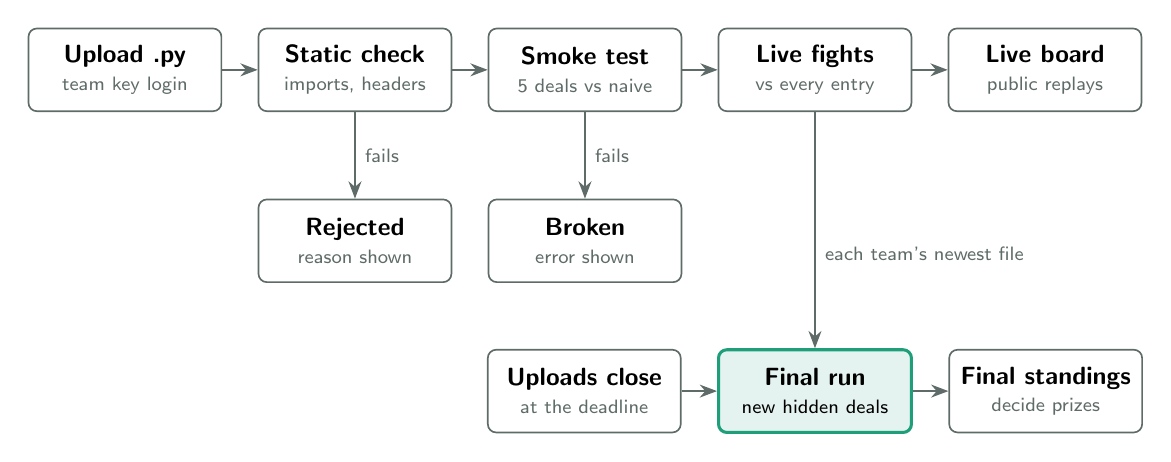
\begin{tikzpicture}[
  font=\sffamily\small,
  box/.style={draw=quiet, rounded corners=3pt, minimum width=2.45cm, minimum height=1.05cm,
              align=center, line width=0.6pt},
  hot/.style={box, draw=mint, fill=mint!12, line width=1.1pt},
  arr/.style={-{Stealth[length=2.2mm]}, draw=quiet, line width=0.6pt},
  lab/.style={font=\sffamily\scriptsize, text=quiet},
  node distance=0.45cm and 0.45cm]
  \node[box] (up) {\textbf{Upload .py}\\[-1pt]{\scriptsize\color{quiet}team key login}};
  \node[box, right=of up] (chk) {\textbf{Static check}\\[-1pt]{\scriptsize\color{quiet}imports, headers}};
  \node[box, right=of chk] (smk) {\textbf{Smoke test}\\[-1pt]{\scriptsize\color{quiet}5 deals vs naive}};
  \node[box, right=of smk] (live) {\textbf{Live fights}\\[-1pt]{\scriptsize\color{quiet}vs every entry}};
  \node[box, right=of live] (brd) {\textbf{Live board}\\[-1pt]{\scriptsize\color{quiet}public replays}};
  \node[box, below=1.1cm of chk] (rej) {\textbf{Rejected}\\[-1pt]{\scriptsize\color{quiet}reason shown}};
  \node[box, below=1.1cm of smk] (brk) {\textbf{Broken}\\[-1pt]{\scriptsize\color{quiet}error shown}};
  \node[hot, below=3.0cm of live] (fin) {\textbf{Final run}\\[-1pt]{\scriptsize new hidden deals}};
  \node[box, left=of fin] (cls) {\textbf{Uploads close}\\[-1pt]{\scriptsize\color{quiet}at the deadline}};
  \node[box, right=of fin] (std) {\textbf{Final standings}\\[-1pt]{\scriptsize\color{quiet}decide prizes}};
  \draw[arr] (up) -- (chk);
  \draw[arr] (chk) -- (smk);
  \draw[arr] (smk) -- (live);
  \draw[arr] (live) -- (brd);
  \draw[arr] (chk) -- node[lab, right] {fails} (rej);
  \draw[arr] (smk) -- node[lab, right] {fails} (brk);
  \draw[arr] (live) -- node[lab, right, pos=0.6] {each team's newest file} (fin);
  \draw[arr] (cls) -- (fin);
  \draw[arr] (fin) -- (std);
\end{tikzpicture}

{\small\color{quiet}Figure 1. The submission pipeline. Only the final run on hidden deals
decides the ranking.}
\end{center}

A failed upload shows its reason at once and does not count against the 10-minute upload
limit. Live fights use one hidden seed and the final uses a different one, so nobody can tune
to the board.

\begin{center}
\begin{tabularx}{\linewidth}{@{}l l L@{}}
\toprule
\textbf{Page} & \textbf{Who sees it} & \textbf{What it shows} \\
\midrule
Standings (home) & Everyone & Live board ranked by score, with PnL per deal, fights won and version; the
  final table on top once it is run; latest fights \\
Team page & Everyone & That team's head-to-head result against every other entry \\
Fight replay & Everyone & The first deal of a fight both ways round: hands, board, moves,
  prices, trades, final PnL \\
Submit & That team only & Upload form, every upload with its status and reason, any timeouts
  or crashes in its fights \\
Kit & Everyone & Zip of the starter bot, house bots, engine, backtester and problem statement \\
\bottomrule
\end{tabularx}
\end{center}

\textbf{Safety.} Every submission runs in its own locked-down process: no files, no network,
no imports outside the allowed list, 50\,ms per call, a memory cap, and a full wipe between
deals. The engine's cards live in a different process, so a bot cannot read them.

\textbf{House bots.} \code{naive}, \code{reader} and \code{sharp} appear on the board, greyed
out, as benchmarks. They do not take a rank.

% ═════════════════════════════════════════════════════════
\section{Timeline and mentors}

The arena opens at kickoff on Monday 5 October and closes on Thursday 8 October, when the final
is run and the results are announced.

\begin{center}
\begin{tabularx}{\linewidth}{@{}>{\bfseries}l L L L@{}}
\toprule
\textbf{Day} & \textbf{What happens} & \textbf{Milestone for each team} & \textbf{Organisers do} \\
\midrule
Mon 5 Oct & Kickoff: the game, the kit, meet your mentor. Arena opens & Run
  \code{backtester.py -{}-show} and explain one deal end to end & Send team keys; post the arena
  link and kit \\
Tue 6 Oct & Mentor check-in 1 & A bot that beats \code{naive} and is on the live board &
  Watch for broken uploads; answer rule questions \\
Wed 7 Oct & Mentor check-in 2 & Beats \code{reader}; knows where it loses PnL & Announce the
  exact deadline again \\
Thu 8 Oct & Uploads close at \TBD{time}. Final run; results at \TBD{time, venue} & Newest
  upload is the one they want & Run the final, back up the data, present results with replays \\
\bottomrule
\end{tabularx}
\end{center}

\textbf{Mentors} look after 3 to 4 teams each and hold a 30-minute check-in with every team on
Tuesday and Wednesday.

\begin{center}
\begin{tabularx}{\linewidth}{@{}LL@{}}
\toprule
\textbf{Mentors may} & \textbf{Mentors may not} \\
\midrule
Explain the rules, probability, card counting and the engine & Write or edit a team's bot \\
Ask ``why?'' until the team finds its own bug & Suggest specific numbers, weights or thresholds \\
Point to the problem statement, house bots and replays & Pass one team's ideas or numbers to another \\
Show how to run a fair test (1,000 deals, several seeds) & Run a team's tuning for them \\
\bottomrule
\end{tabularx}
\end{center}

Before kickoff every mentor should read the problem statement, play through
\code{python backtester.py -{}-show}, and be able to explain three things without notes: why the
unseen cards are worth the average unseen rank, why a maker's price leaks its hand, and why 100
deals prove nothing. Suspected copying, or a team that cannot explain its own code, goes to the
coordinators, not to the team.

% ═════════════════════════════════════════════════════════
\section{Operations}

The arena needs no AWS: one machine that stays on for four days and a public link. The
recommended setup is a club laptop with a free Cloudflare tunnel; an Oracle Cloud free VM is
the sturdier alternative.

\begin{center}
\begin{tabularx}{\linewidth}{@{}L l l L@{}}
\toprule
\textbf{Option} & \textbf{Cost} & \textbf{Setup} & \textbf{Watch out for} \\
\midrule
\textbf{Club laptop + Cloudflare tunnel} (recommended) & Free & 5 min & Must stay on, awake and
  online; the link changes on restart \\
\textbf{Oracle Cloud Always Free VM} or a college server, with Docker & Free & 30 min & Open
  port 80 in the VM firewall \\
\textbf{Railway or Fly.io} from the Dockerfile & A few \$ & 15 min & Attach a volume at
  \code{/data}, or results are lost on redeploy \\
\bottomrule
\end{tabularx}
\end{center}

Do not use Render's free tier: it sleeps when idle and wipes its disk.

\subsection{Setup on the laptop}

\begin{lstlisting}[language=bash]
winget install Cloudflare.cloudflared     # once
cd hiddenhand
python arena.py add-team "Team Name"      # once per team; prints its key
set DEADLINE=2026-10-08T18:00             # uploads close by themselves
python arena.py --tunnel                  # prints the public https link
\end{lstlisting}

Send each team its key privately and post the link on the group. Set the laptop never to sleep,
and allow Python through the firewall if Windows asks. \code{python arena.py teams} lists every
team and key again.

\textbf{Settings} (environment variables, all optional): \code{DEADLINE} closes uploads;
\code{DEALS} $=200$ deals each way per live fight; \code{FINAL\_DEALS} $=500$;
\code{COOLDOWN} $=600$ seconds between uploads; \code{WORKERS} $=$ fights run at once (CPU
cores minus one).

\subsection{Last day}

\begin{enumerate}
  \item At the deadline uploads close automatically.
  \item Run \code{python arena.py final} on the arena machine. With 30 teams that is about 500
        fights; with 3 workers allow 15 to 30 minutes.
  \item The final table appears at the top of the site at once. Open the top fights' replays
        for the results presentation.
  \item Copy the \code{arena\_data} folder somewhere safe. It holds every upload and every result.
\end{enumerate}

The full guide, including the Docker commands, is \code{DEPLOY.md} in the \code{hiddenhand/}
folder.

% ═════════════════════════════════════════════════════════
\section{Open items}\label{sec:open}

The game, the problem statement and the site are final. These details must be filled in before
the problem statement goes out; each is marked \TBD{\dots} in this document and in the README.

\begin{itemize}[label=$\square$]
  \item Choose the hosting option, start the arena and put its link in the problem statement
  \item Exact upload deadline on Thu 8 Oct (also set as \code{DEADLINE})
  \item Results announcement time and venue
  \item Registration link and registration deadline
  \item Prizes
  \item Coordinator names and phone numbers
  \item Mentor list and team-to-mentor assignment
  \item One team key per registered team, sent privately
  \item Retire the old Divided Oracle problem statement and the \code{freshers-ps/} folder
\end{itemize}

\end{document}
